\documentclass{article}
\usepackage{indentfirst}
\usepackage{ctex}
\usepackage{geometry}
\usepackage{enumerate}
\usepackage{amssymb, amsmath}
\usepackage{graphicx, subfigure}
\geometry{left=3.17cm,right=3.17cm,top=2.54cm,bottom=2.54cm} % 页边距

\begin{document}
	
\begin{figure}[htbp]
	\centering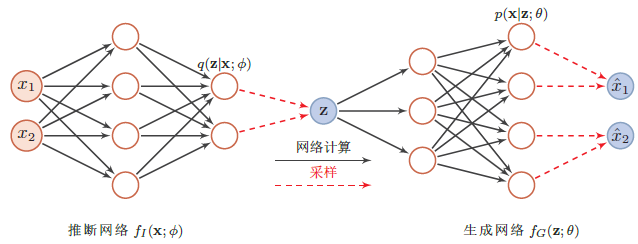
\includegraphics[height=5cm]{arch.png}
	\caption{变分自编码器的网络结构}
	\label{fig:arch}
\end{figure}

推断网络和生成网络的目标都是最大化证据下界$ELBO$(\emph{evidence lower bound})

\begin{equation}
\mathcal{L}(\theta,\phi;\mathbf{x})=\mathbb{E}_{\mathbf{z}\sim q(\mathbf{z}|\mathbf{x};\theta)}[\log p(\mathbf{x}|\mathbf{z};\theta)]-D_{KL}[q(\mathbf{z}|\mathbf{x};\phi)\lVert p(\mathbf{z};\theta)] \label{eq:ELBO}
\end{equation}

其中,$\log p(\mathbf{x}|\mathbf{z};\theta)$是边缘对数似然(\emph{marginal log likehood}), $ELBO$也叫做“边缘对数似然的下界(\emph{a lower bound on the marginal log likehood})” \par
最大化$ELBO$等价于最大化Eq.(\ref{eq:ELBO})中的期望$\mathbb{E}$、最小化$D_{KL}$. \par
期望$\mathbb{E}$一般通过采样的方式进行计算。对于每个样本$\mathbf{x}$,根据$q(\mathbf{z}|\mathbf{x};\phi)$采集$M$个$\mathbf{z}^{(m)}$,

\begin{equation}
\mathbb{E}_{\mathbf{z}\sim q(\mathbf{z}|\mathbf{x};\theta)}[\log p(\mathbf{x}|\mathbf{z};\theta)]\approx \frac{1}{M}\sum_{m=1}^{M}\log p(\mathbf{x}|\mathbf{z}^{(m)};\theta) \label{eq:E}
\end{equation}

\par
如果采用随机梯度(\emph{stochastic gradients})方法,每次从数据集中采集一个$\mathbf{x}$,然后根据$q(\mathbf{z}|\mathbf{x};\phi)$采集一个隐变量$\mathbf{z}$,则目标函数变为

\begin{equation}
\mathcal{L}(\theta,\phi;\mathbf{x})=\log p(\mathbf{x}|\mathbf{z};\theta)-D_{KL}[q(\mathbf{z}|\mathbf{x};\phi)\lVert p(\mathbf{z};\theta)] \label{eq:ELBO2}
\end{equation}

即:最大化$\log p(\mathbf{x}|\mathbf{z};\theta) \Rightarrow$最小化$-\log p(\mathbf{x}|\mathbf{z};\theta)$\\

$\therefore$ 训练目标:最小化$\underbrace{-\log p(\mathbf{x}|\mathbf{z};\theta)}_{generation\_loss}$和$\underbrace{D_{KL}}_{latent\_loss}$\\

Auto-Encoding Variational Bayes - Appendix C.1给出了$\log p(\mathbf{x}|\mathbf{z};\theta)$的计算公式。公式中的$\mathbf{y}$就是代码中的\textbf{x\_reconstr\_mean}. Appendix B给出了$D_{KL}$的计算公式。 其他参数的计算公式的出处亦注释在代码中。

代码中定义encoder network和decoder network时的\textbf{layer\_2}相当于论文Auto-Encoding Variational Bayes给出的众多公式中的$\mathbf{h}$. 论文的示例网络MLP只有一层隐藏层,而代码中定义了两层隐藏层,因此需要一个转移方程\textbf{transfer\_func}来完成层与层之间的转移.

\end{document}
 